% Schematic single-dot blockade map for locally linear gate response.
% Equal adjacent addition gaps and beta=1/2 give symmetric diamonds.
% Positive V_b means mu_S > mu_D, as in the chapter's convention.
\begingroup
\definecolor{diamondGate}{HTML}{0072B2}
\definecolor{diamondBias}{HTML}{D55E00}
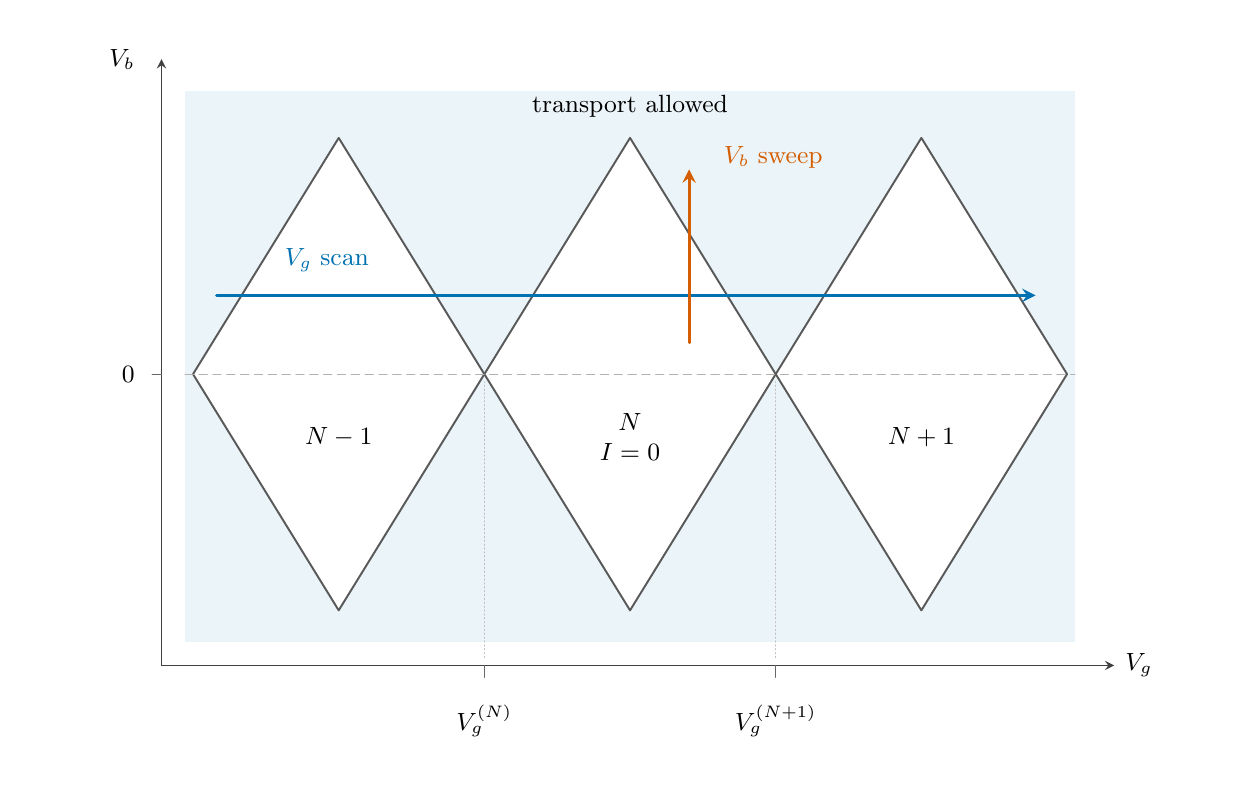
\begin{tikzpicture}[
 x=1mm,y=1mm,>=stealth,line cap=round,line join=round,
 every node/.style={font=\small,inner sep=1pt}
]
 \path[use as bounding box] (0,3) rectangle (150,96);

 % Pale regions admit charge transfer; white diamonds are blocked.
 \fill[diamondGate!8] (20,18) rectangle (133,88);
 \foreach \diamondLeft in {21,58,95}{
  \path[fill=white,draw=black!65,line width=0.7pt]
       (\diamondLeft,52)
       --({\diamondLeft+18.5},82)
       --({\diamondLeft+37},52)
       --({\diamondLeft+18.5},22)--cycle;
 }
 \draw[black!30,densely dashed,line width=0.4pt]
      (20,52)--(133,52);
 \node at (39.5,44) {$N-1$};
 \node[align=center] at (76.5,44) {$N$\\$I=0$};
 \node at (113.5,44) {$N+1$};

 % Two independent scan directions in voltage space.
 \draw[->,diamondGate,line width=1.1pt] (24,62)--(128,62);
 \node[text=diamondGate] at (38,66.5) {$V_g$ scan};
 \draw[->,diamondBias,line width=1.1pt] (84,56)--(84,78);
 \node[text=diamondBias,anchor=west] at (88,79.5) {$V_b$ sweep};
 \node at (76.5,86) {transport allowed};

 % Coordinate axes and zero-bias transition positions.
 \draw[->,black!75,line width=0.5pt] (17,15)--(138,15);
 \draw[->,black!75,line width=0.5pt] (17,15)--(17,92);
 \node[anchor=west] at (139,15) {$V_g$};
 \node[anchor=east] at (14,92) {$V_b$};
 \draw[black!60,line width=0.4pt] (15.8,52)--(17,52);
 \node[anchor=east] at (14,52) {$0$};
 \foreach \tickX in {58,95}{
  \draw[black!25,densely dotted,line width=0.4pt]
       (\tickX,16)--(\tickX,51);
  \draw[black!60,line width=0.4pt]
       (\tickX,15)--(\tickX,13.5);
 }
 \node at (58,8) {$V_g^{(N)}$};
 \node at (95,8) {$V_g^{(N+1)}$};
\end{tikzpicture}
\endgroup
